\documentclass[10pt,journal,compsoc]{IEEEtran}


% *** CITATION PACKAGES ***
\ifCLASSOPTIONcompsoc
  % IEEE Computer Society needs nocompress option
  % requires cite.sty v4.0 or later (November 2003)
  \usepackage[nocompress]{cite}
\else
  % normal IEEE
  \usepackage{cite}
\fi


% *** GRAPHICS RELATED PACKAGES ***
\ifCLASSINFOpdf
  \usepackage{graphicx}
  % declare the path(s) where your graphic files are
  \graphicspath{{Figures/}{Other_Folder/}}
  % and their extensions so you won't have to specify these with
  % every instance of \includegraphics
  \DeclareGraphicsExtensions{.pdf,.jpeg,.png}
\else
  % or other class option (dvipsone, dvipdf, if not using dvips). graphicx
  % will default to the driver specified in the system graphics.cfg if no
  % driver is specified.
  % \usepackage[dvips]{graphicx}
  % declare the path(s) where your graphic files are
  % \graphicspath{{../eps/}}
  % and their extensions so you won't have to specify these with
  % every instance of \includegraphics
  % \DeclareGraphicsExtensions{.eps}
\fi


% *** SUBFIGURE PACKAGES ***
\ifCLASSOPTIONcompsoc
 \usepackage[caption=false,font=footnotesize,labelfont=sf,textfont=sf]{subfig}
\else
 \usepackage[caption=false,font=footnotesize]{subfig}
\fi


% *** PDF, URL AND HYPERLINK PACKAGES ***
\usepackage{url}
% correct bad hyphenation here
\usepackage{hyperref}


\hyphenation{op-tical net-works semi-conduc-tor}


\begin{document}
%
\title{Concurrency and Parallelism Report}

\author{Pedro~Madeira~\IEEEmembership{52464,}
        António~Pereira~\IEEEmembership{55416,}
        and~Diogo~Lages~\IEEEmembership{55951}% <-this % stops a space
        
\IEEEcompsocitemizethanks{\IEEEcompsocthanksitem All the students were with the Department of Computer Science, NOVA School of Science and Technology.\protect\\
% note need leading \protect in front of \\ to get a newline within \thanks as
% \\ is fragile and will error, could use \hfil\break instead.
E-mail Pedro Madeira: pv.madeira@campus.fct.unl.pt\\
E-mail António Pereira: adm.pereira@campus.fct.unl.pt\\
E-mail Diogo Lages: d.lages@campus.fct.unl.pt}\\
}

% The paper headers
\markboth{Concurrency and Parallelism Report, June 2021}%
{Shell \MakeLowercase{\textit{et al.}}: Bare Demo of IEEEtran.cls for Computer Society Journals}

\IEEEtitleabstractindextext{%
\begin{abstract}
The evolution of computing technology enters an era of advances in processor architectures, such as multi-core, increasing the complexity of parallel computing systems. Thus, multi-core features a variety of parallel programming languages for running parallel programs being OpenMP one of the most successful libraries to apply. It is an application program interface (API) for parallel programming model of shared memory multiprocessors. Due to this progression in architectures and their complexity, the constant analysis and evaluation of the performance of OpenMP builds, kernels and applications on multi-core systems has become very significant, since performance consists of gathering all information about the execution characteristics of a program. There are three interfacing software layers used to classify the performance: the instrumentation layer, which defines the evaluated performance events, the classification or measurement layer, which determines which performance event is, in reality, caught and how the tool will measure it, and the analysis layer, which processes the performance data and compiles it into a structure that can be displayed in performance tools. In this paper, it is given a solution for the Concurrency and Parallelism Project problem and the structure for testing, analyzing and evaluating it.
\end{abstract}

% Note that keywords are not normally used for peerreview papers.
\begin{IEEEkeywords}
OpenMP, Parallelism, Analysis
\end{IEEEkeywords}}


% make the title area
\maketitle

\IEEEdisplaynontitleabstractindextext

\IEEEpeerreviewmaketitle

\IEEEraisesectionheading{\section{Introduction}\label{sec:introduction}}


\IEEEPARstart{T}{he} advance of modern computing technology brought to us the necessity to upgrade processor architectures contributing to the enlargement of complexity of parallel systems. Within the multi-core architecture there are varieties of parallel languages that can be utilized to run the parallel programs \cite{surveyTools}. The OpenMP, in comparison with other parallel languages, shows a lot more efficacy when used with multi-core architectures.\\
In this last years, with this computing enhancement, the need of learning, and being comfortable with the environment and performance of OpenMP has been increasing. However,this requirement will guide us to the encounter of new problems and challenges, within the "OpenMP parallelization world", which can only be analyzed and evaluated by the platform and the compiler specific mechanism \cite{surveyTools} since there is, still, no interface to analyze the performance of OpenMP.\\
Our goal in this project is to parallelize a sequential program using the OpenMP libraries incorporated with C/C++ and to analyze our solution testing the parallelization with different values, such as the number of threads used in our methods, the input values, etc.\\
Our approach to the project in general was based on Bloom's Taxonomy Pyramid, which is a set of hierarchical models to classify and specify the knowledge levels. There are six levels in Bloom's Pyramid: remembering, understanding, applying, analyzing, evaluating, and creating, where each one depends on the one below.\\

\begin{center}
    \begin{figure}[h!]
        \centering{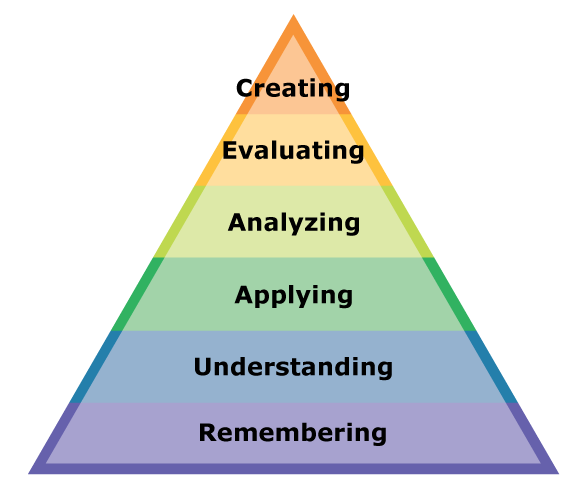
\includegraphics[width=4cm]{Bloom's Pyramid.png}}
        \caption{Knowledge Levels of Bloom's Pyramid}
        \centering{\label{fig}}
    \end{figure}
\end{center}

We figured that following this steps would be the best way to start our project so the first stage was to remember the theory given in the course classes and we even checked all the course subjects that we considered important to the realization of the project. The next steps were to understand everything that was being given to us (initial code, utterance, tests, report format, etc) and starting to apply what was necessary for the parallelization of the program. The next two phases (analyzing and evaluating) were done simultaneously, as we started taking note of the responses from our parallel program as soon as we started testing our solution. The last stage of the pyramid was implemented after realizing what were the pros and cons of our parallel solution and figuring out if it was necessary to change something in our program in order to get a better solution.

%\hfill June 06, 2021

\section{Beforehand concepts}
We're gonna explain some concepts before going further. These are for analysis and evaluation purposes.

\subsection{Class contents}
\begin{itemize}
    \item \textbf{Speedup} is given by the ratio of the time it takes the sequential version to execute for the time it takes the parallel version to execute.
    \item \textbf{Efficiency} is given by the ratio of the Speedup for the number of threads that ran during the parallel program.
    \item \textbf{Cost} is given by the time of the parallel execution times the number of threads that ran during it's execution.
    \item \textbf{Amdahl's Law} gives us an upper bound for the speedup, assuming that we want to compute the same work as in the sequential version. This assumption is correct because increasing the work won't help us in this project, our goal is to decrease the time it takes to compute the \underline{same amount of work}.
\end{itemize}

\subsection{Concept application in this project}
The speedup is an obvious choice for measuring how faster our parallel version is than the sequential. Efficiency and cost are used for checking if our solution is optimal. \textbf{Amdahl's Law isn't applied directly. It's more of a curiosity after getting our results to define an upper bound for the speedup and compute the sequential fraction of the algorithm. LEMBRAR DE FAZER VÁRIOS TESTES: COM O MESMO MÉTODO MAS COM O NÚMERO DE THREADS INCREASING. ISTO É PORQUE À MEDIDA QUE SE AUMENTA O NR DE THREADS A SPEEDUP VAI ATENUANDO} 
\begin{center}
\textit{\\"A parallel algorithm is cost-optimal if\\ Efficiency = 100\% and Cost = Sequential Time"}
\end{center}

\section{Analysis and approach}

\subsection{Code analysis}
Fazer secções para cada ponto do projeto? 4.x até 4.y?

\subsection{Approach to OpenMP solution}
\begin{itemize}
    \item Tentámos isto - não funcionou porque - pôr gráfico de resultados
    \item Tentámos isto - também não deu porque - pôr gráfico de resultados
    \item Tentámos isto - das 3 foi a melhor - pôr gráfico de resultados comparando com as outas tentativas
\end{itemize}

\section{Evaluation/tests and corrections}
We tested ...

\subsection{Python script}
We made a script....
We also used scripts from Piazza...

\subsection{Changes made}
What needed to be changed

\subsection{Final solution}
Final code algorithm

\section{Results}
MAIS, MUITO MAIS GRÁFICOS

\subsection{Performance}
Análise dos resultados


\section{Conclusion}
The conclusion goes here.


% use section* for acknowledgment
\ifCLASSOPTIONcompsoc
  % The Computer Society usually uses the plural form
  \section*{Acknowledgments}
\else
  % regular IEEE prefers the singular form
  \section*{Acknowledgment}
\fi


We would like to thank:
\begin{itemize}
    \item Everyone that helped us indirectly through Piazza workspace, namely on threads @77 (João Antão and his colleagues from Group 15, Jorge Coelho)...
    \item Group 40 which helped us repairing some errors we had in our code 
\end{itemize}

% Can use something like this to put references on a page
% by themselves when using endfloat and the captionsoff option.
\ifCLASSOPTIONcaptionsoff
  \newpage
\fi


\begin{thebibliography}{1}

\bibitem{surveyTools}
Mubrak S. Mohsen, Rosni Abdullah, and Yong M. Teo, \emph{A Survey on Performance Tools for OpenMP}, 2009, p.1

\end{thebibliography}

% that's all folks
\end{document}